\section{Connect to eduroam}	\label{sec:run-eduroam}
	 To re-run the project, you have to connect your Raspberry Pi with ``eduroam'' network at The Univeristy of Alabama. Now, if you have freshly install the Raspberry Pi OS, then you need to run the script called \textbf{``config\_eduroam.sh''}, which can be found \href{https://github.com/TrupeshKumarPatel/IoT_RaspberryPi/tree/main/source_code/eduroam_config}{here}. 
	 
\subsection{Configure Raspberry Pi for eduroam}
		\begin{itemize}[leftmargin=1.8cm]
			\item[\textbf{Step 1:}] Login to the Raspberry Pi as user ``pi'' %(\textbf{Note:} You can follow steps from \hyperref[subsubsec:ssh]{Section \ref{subsubsec:ssh}}.)
			\item[\textbf{Step 2:}] Type command ``{\fontfamily{cmtt}\selectfont{git clone https://github\\.com/TrupeshKumarPatel/IoT\_RaspberryPi.\\git}}''\\
				\begin{minipage}{\textwidth}
					\vspace{2mm}
					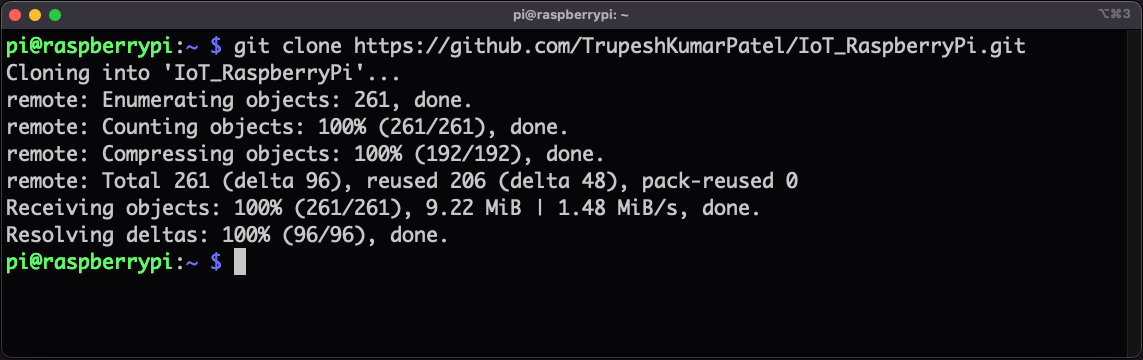
\includegraphics[scale=0.17]{Images/raspberry_pi/eduroam_config/clone_git.png}
					\vspace{2mm}
				\end{minipage}
			\item[\textbf{Step 3:}] Type command ``{\fontfamily{cmtt}\selectfont{sudo su}}'' ~\danger\textbf{NOTE} ~This com\\mand to get sudo access to Raspberry Pi \danger\\
				\begin{minipage}{\textwidth}
					\vspace{2mm}
					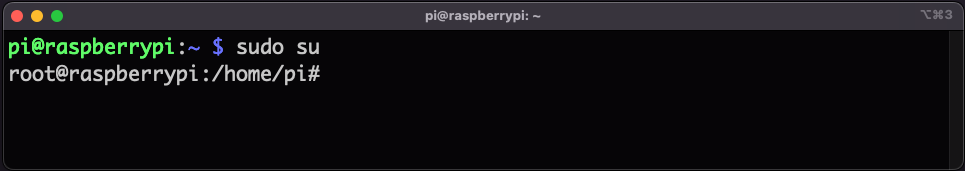
\includegraphics[scale=0.2]{Images/raspberry_pi/eduroam_config/sudo_login.png}
					\vspace{2mm}
				\end{minipage}
			\item[\textbf{Step 4:}] Type command ``{\fontfamily{cmtt}\selectfont{chmod +x IoT\_Raspberry\\Pi/source\_code/eduroam\_config/config\\\_eduroam.sh}}''\\
				\begin{minipage}{\textwidth}
					\vspace{2mm}
					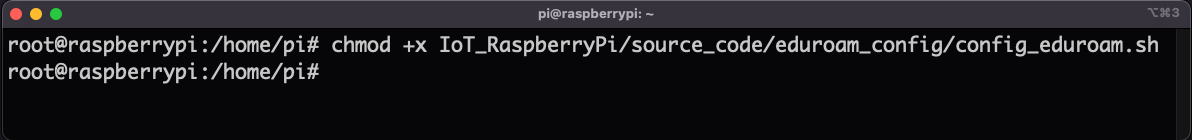
\includegraphics[scale=0.16]{Images/raspberry_pi/eduroam_config/permission_x.png}
					\vspace{2mm}
				\end{minipage}
			\item[\textbf{Step 5:}] Type command ``{\fontfamily{cmtt}\selectfont{./IoT\_RaspberryPi/sourc\\e\_code/eduroam\_c\\onfig/config\_eduroam.sh}}''
			\item[\textbf{Step 6:}] Enter your crimson email address
			\item[\textbf{Step 7:}] Enter your crimson password\\
				\begin{minipage}{\textwidth}
					\vspace{2mm}
					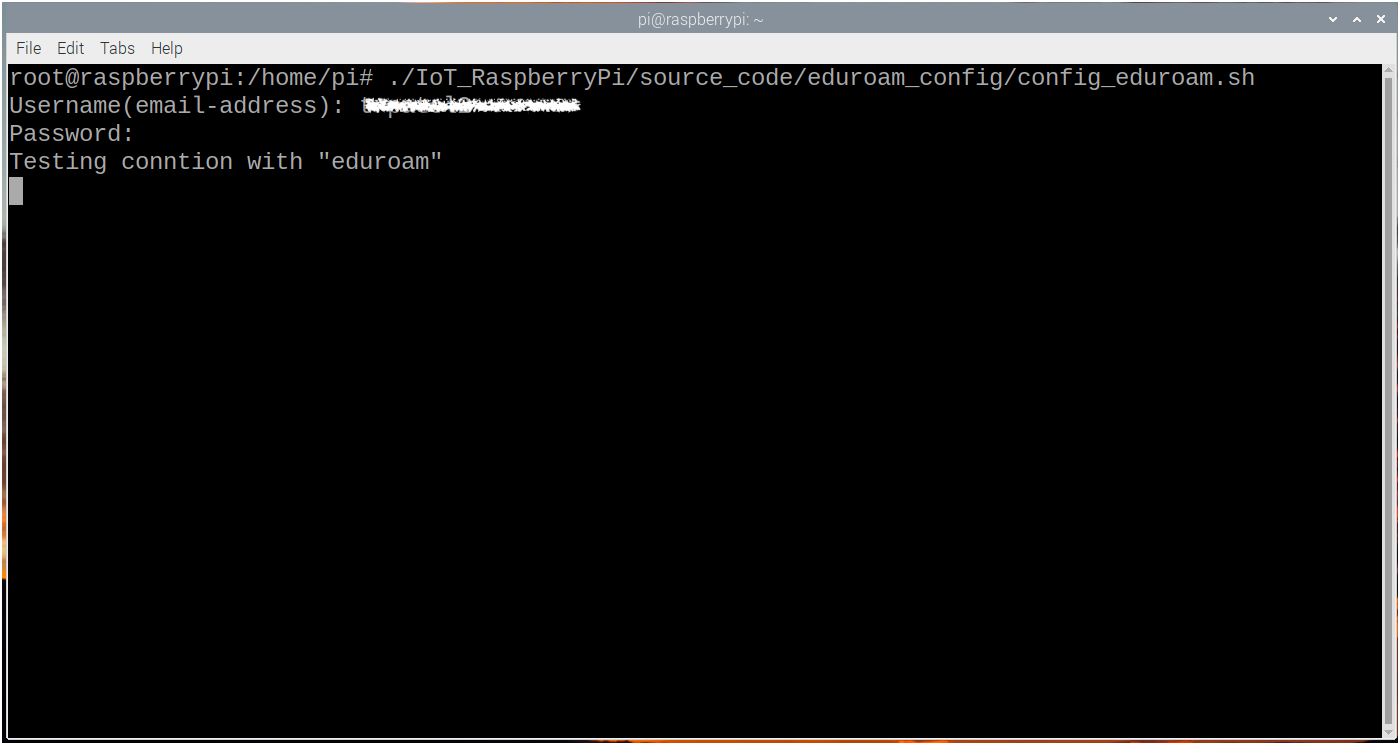
\includegraphics[scale=0.14]{Images/raspberry_pi/eduroam_config/run_eduroam_conf.png}
					\vspace{2mm}
				\end{minipage}
			\item[\textbf{Step 8:}] Now wait for your Raspberry Pi to restart
		\end{itemize}